% MolSSD Project Mind Map
% Compile with: pdflatex mindmap.tex
\documentclass[border=15mm]{standalone}

\usepackage[T1]{fontenc}
\usepackage{lmodern}
\usepackage{tikz}
\usetikzlibrary{mindmap,backgrounds,positioning}

% colour palette
\definecolor{coreOrange}{HTML}{E8590C}
\definecolor{brTheory}{HTML}{1971C2}
\definecolor{brMath}{HTML}{2F9E44}
\definecolor{brArch}{HTML}{9C36B5}
\definecolor{brScale}{HTML}{E67700}
\definecolor{brData}{HTML}{0CA678}
\definecolor{brUV}{HTML}{D6336C}
\definecolor{brPipe}{HTML}{4263EB}
\definecolor{brGaps}{HTML}{F76707}
\definecolor{brBase}{HTML}{495057}

\begin{document}

% Title
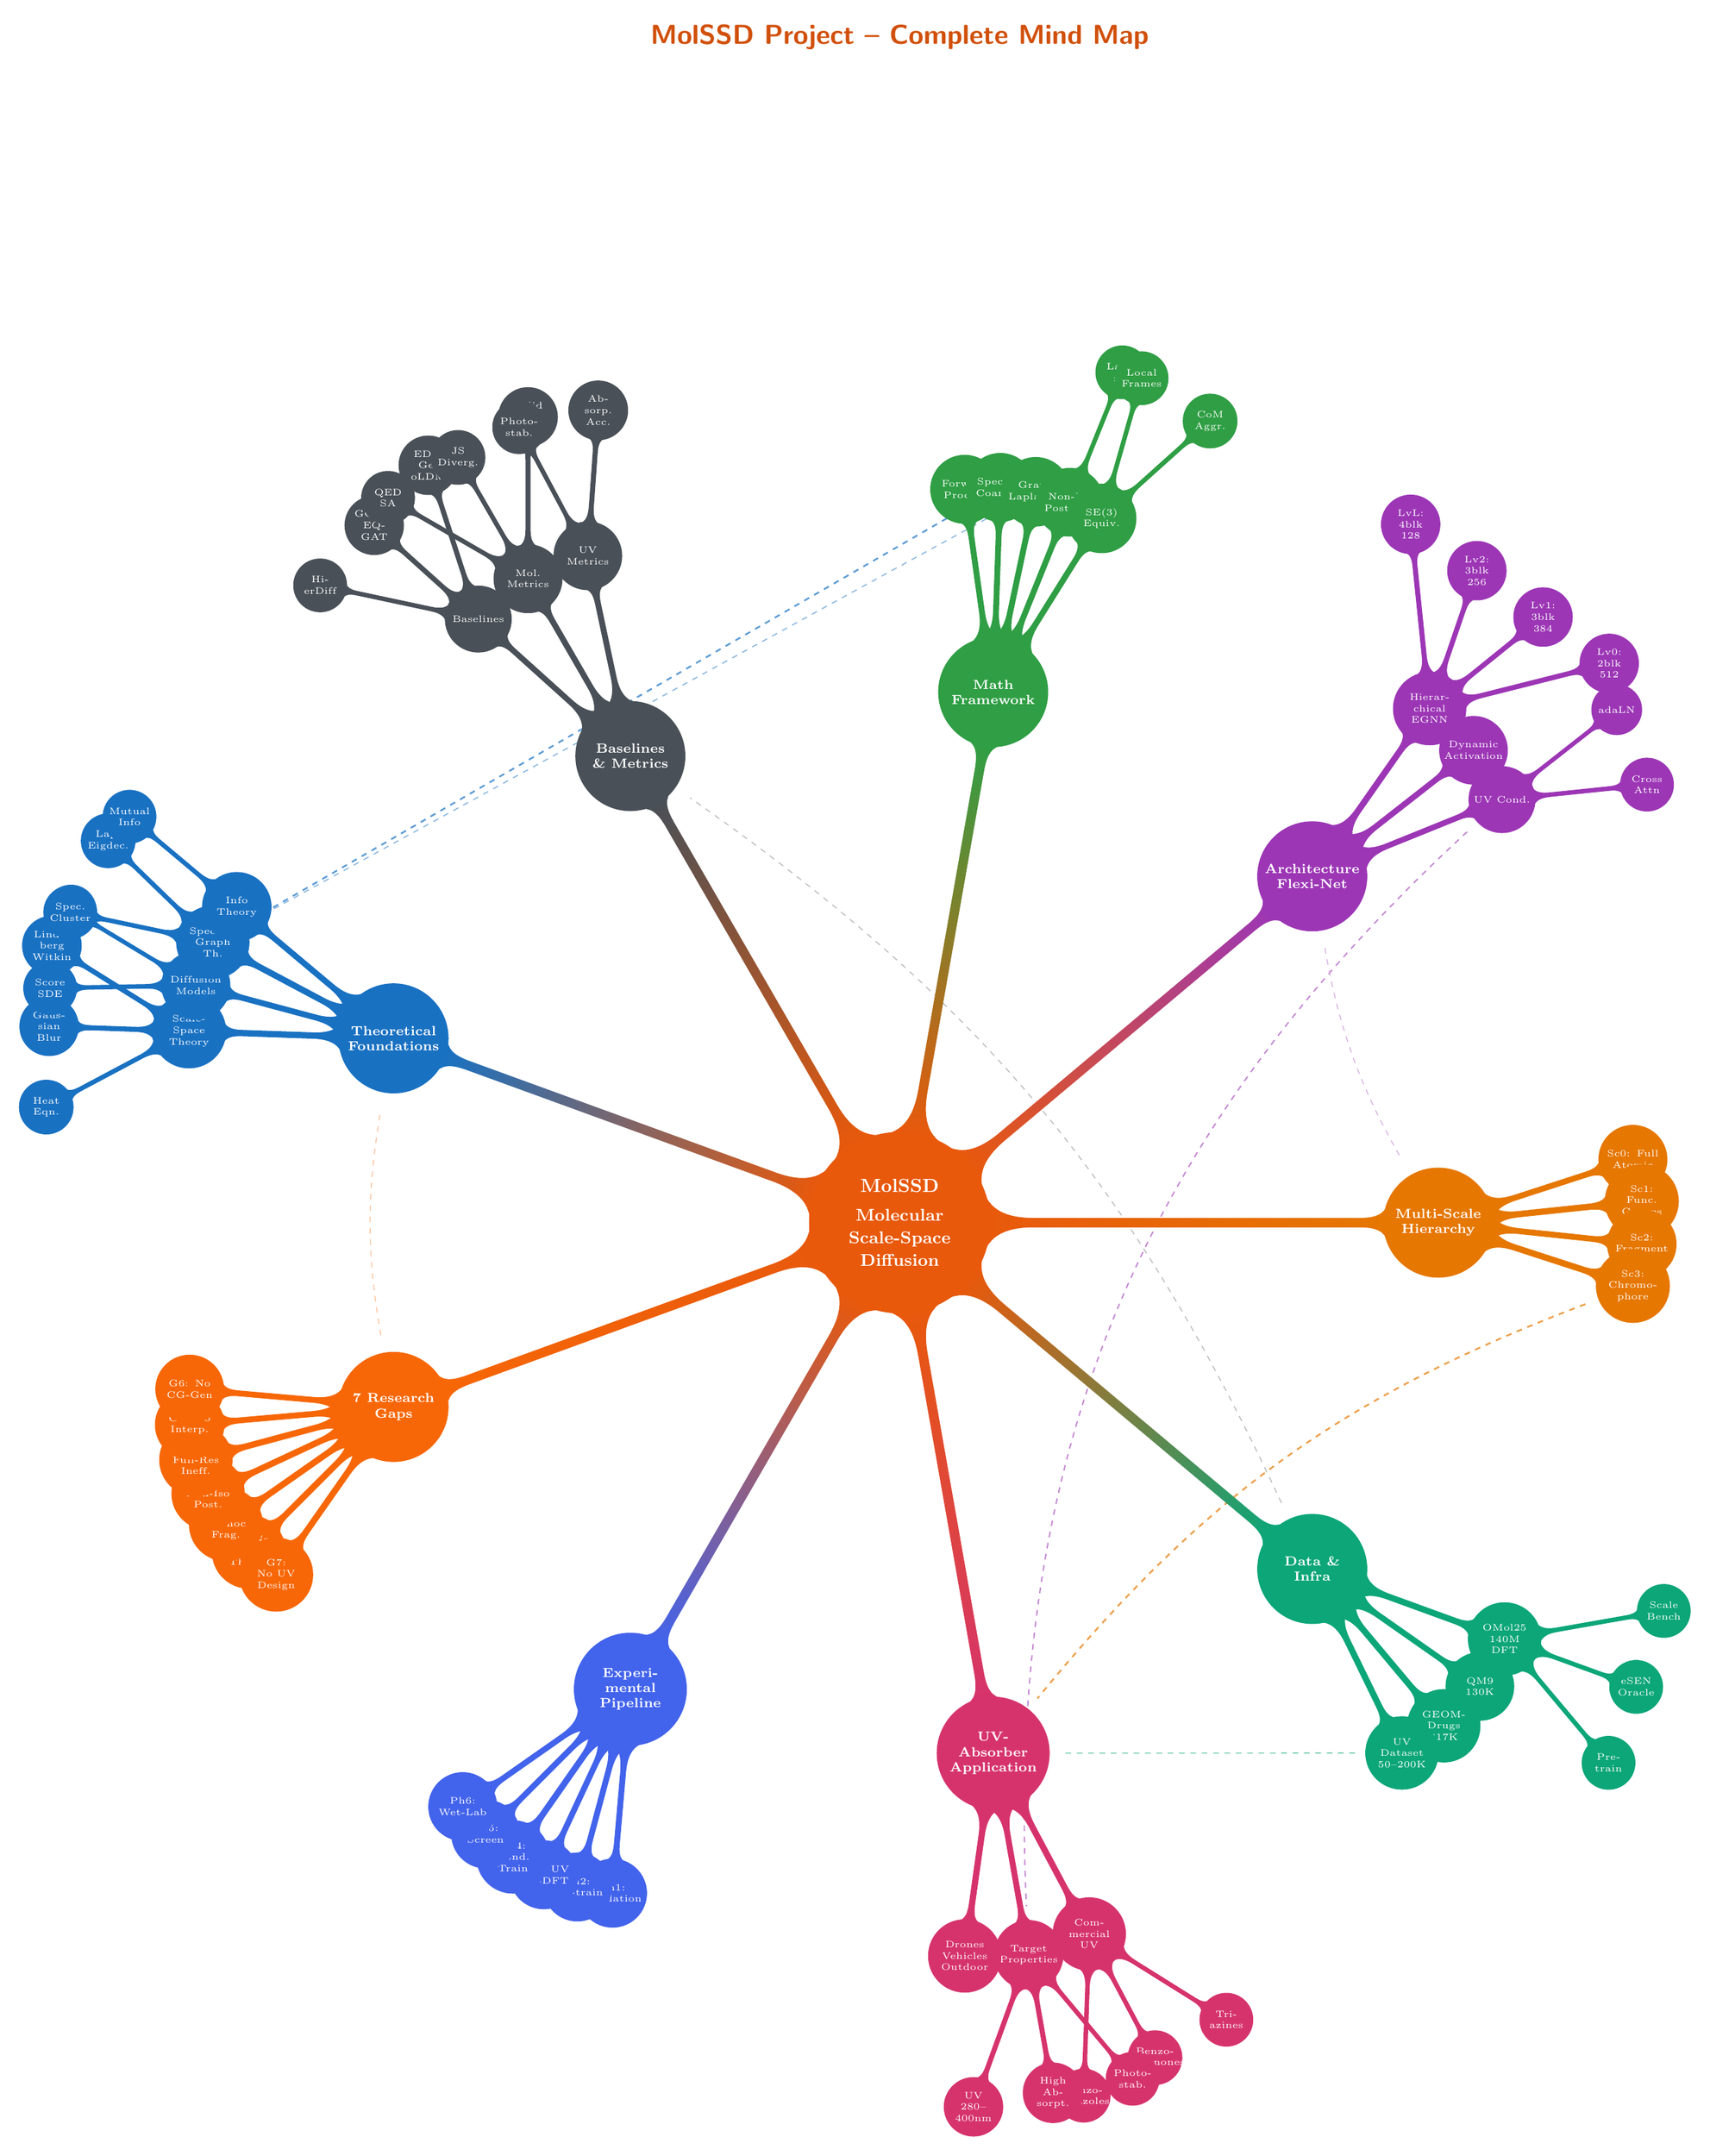
\begin{tikzpicture}

\node[font=\Large\bfseries\sffamily, text=coreOrange!90!black] at (0,22)
  {MolSSD Project -- Complete Mind Map};

\begin{scope}[
  mindmap,
  every node/.style={concept, execute at begin node=\hskip0pt},
  grow cyclic,
  text=white,
  concept color=coreOrange,
  level 1/.append style={
    level distance=10cm,
    sibling angle=40,
    font=\scriptsize\bfseries,
    minimum size=2.0cm,
    text width=1.8cm,
  },
  level 2/.append style={
    level distance=3.8cm,
    sibling angle=30,
    font=\tiny,
    minimum size=1.2cm,
    text width=1.1cm,
  },
  level 3/.append style={
    level distance=2.6cm,
    sibling angle=28,
    font=\tiny,
    minimum size=0.9cm,
    text width=0.8cm,
  },
]

% CENTRAL NODE
\node [font=\normalsize\bfseries, minimum size=3.2cm, text width=2.8cm]
  {MolSSD\\[3pt]{\small Molecular}\\{\small Scale-Space}\\{\small Diffusion}}
%
% ===============================================================
% 9 branches at even 40-degree spacing: 0, 40, 80, 120, 160,
% 200, 240, 280, 320.  Children stay within +-25 deg of parent.
% ===============================================================
%
% BRANCH 1 - Multi-Scale Hierarchy  (0 deg, right)
  child [concept color=brScale, grow=0] {
    node (hierarchy) {Multi-Scale Hierarchy}
    child [grow=18] {
      node {Sc0: Full Atomic}
    }
    child [grow=6] {
      node {Sc1: Func.\ Groups}
    }
    child [grow=-6] {
      node {Sc2: Fragment}
    }
    child [grow=-18] {
      node (chromo) {Sc3: Chromo\-phore}
    }
  }
%
% BRANCH 2 - Architecture  (40 deg, upper-right)
  child [concept color=brArch, grow=40] {
    node (arch) {Architecture Flexi-Net}
    child [grow=55] {
      node {Hierarchical EGNN}
      child { node {Lv0: 2blk 512} }
      child { node {Lv1: 3blk 384} }
      child { node {Lv2: 3blk 256} }
      child { node {LvL: 4blk 128} }
    }
    child [grow=38] {
      node {Dynamic Activation}
    }
    child [grow=22] {
      node (uvcond) {UV Cond.}
      child { node {Cross Attn} }
      child { node {adaLN} }
    }
  }
%
% BRANCH 3 - Mathematical Framework  (80 deg, upper)
  child [concept color=brMath, grow=80] {
    node (math) {Math Framework}
    child [grow=98] {
      node {Forward Process}
    }
    child [grow=88] {
      node (speccoarse) {Spectral Coarsen.}
    }
    child [grow=78] {
      node (graphlap) {Graph Laplacian}
    }
    child [grow=68] {
      node {Non-Iso Posterior}
      child { node {Lanczos} }
    }
    child [grow=58] {
      node {SE(3) Equiv.}
      child { node {CoM Aggr.} }
      child { node {Local Frames} }
    }
  }
%
% BRANCH 4 - Baselines & Metrics  (120 deg, upper-left)
  child [concept color=brBase, grow=120] {
    node (baselines) {Baselines \& Metrics}
    child [grow=138] {
      node {Baselines}
      child { node {EDM GeoLDM} }
      child { node {GCDM EQGAT} }
      child { node {HierDiff} }
    }
    child [grow=120] {
      node {Mol.\ Metrics}
      child { node {Valid Uniq Nov} }
      child { node {JS Diverg.} }
      child { node {QED SA} }
    }
    child [grow=102] {
      node (uvmetrics) {UV Metrics}
      child { node {Absorp.\ Acc.} }
      child { node {Photostab.} }
    }
  }
%
% BRANCH 5 - Theoretical Foundations  (160 deg, left)
  child [concept color=brTheory, grow=160] {
    node (theory) {Theoretical Foundations}
    child [grow=178] {
      node (sst) {Scale-Space Theory}
      child { node {Lindeberg Witkin} }
      child { node {Gaussian Blur} }
      child { node {Heat Eqn.} }
    }
    child [grow=165] {
      node {Diffusion Models}
      child { node {DDPM} }
      child { node {Score SDE} }
    }
    child [grow=152] {
      node (sgt) {Spectral Graph Th.}
      child { node {Lap.\ Eigdec.} }
      child { node {Spec.\ Cluster} }
    }
    child [grow=140] {
      node {Info Theory}
      child { node {Mutual Info} }
    }
  }
%
% BRANCH 6 - Research Gaps  (200 deg, lower-left)
  child [concept color=brGaps, grow=200] {
    node (gaps) {7 Research Gaps}
    child [grow=225] {
      node {G1: No Info-Theory}
    }
    child [grow=215] {
      node {G2: Ad-hoc Frag.}
    }
    child [grow=205] {
      node {G3: Non-Iso Post.}
    }
    child [grow=195] {
      node {G4: Full-Res Ineff.}
    }
    child [grow=185] {
      node {G5: No Interp.}
    }
    child [grow=175] {
      node {G6: No CG-Gen}
    }
    child [grow=235] {
      node {G7: No UV Design}
    }
  }
%
% BRANCH 7 - Experimental Pipeline  (240 deg, lower-left)
  child [concept color=brPipe, grow=240] {
    node (pipe) {Experimental Pipeline}
    child [grow=265] {
      node {Ph1: Validation}
    }
    child [grow=255] {
      node {Ph2: Pre-train}
    }
    child [grow=245] {
      node {Ph3: UV TD-DFT}
    }
    child [grow=235] {
      node {Ph4: Cond.\ Train}
    }
    child [grow=225] {
      node (phase5) {Ph5: Screen}
    }
    child [grow=215] {
      node {Ph6: Wet-Lab}
    }
  }
%
% BRANCH 8 - UV-Absorber Application  (280 deg, lower)
  child [concept color=brUV, grow=280] {
    node (uvapp) {UV-Absorber Application}
    child [grow=298] {
      node {Commercial UV}
      child { node {Benzo\-triazoles} }
      child { node {Benzo\-phenones} }
      child { node {Triazines} }
    }
    child [grow=280] {
      node (uvtarget) {Target Properties}
      child { node {UV 280--400nm} }
      child { node {High Absorpt.} }
      child { node {Photo\-stab.} }
    }
    child [grow=262] {
      node {Drones Vehicles Outdoor}
    }
  }
%
% BRANCH 9 - Data & Infrastructure  (320 deg, lower-right)
  child [concept color=brData, grow=320] {
    node (data) {Data \& Infra}
    child [grow=340] {
      node (omol) {OMol25 140M DFT}
      child { node (pretrain) {Pre-train} }
      child { node {eSEN Oracle} }
      child { node {Scale Bench} }
    }
    child [grow=325] {
      node {QM9 130K}
    }
    child [grow=310] {
      node {GEOM-Drugs 317K}
    }
    child [grow=296] {
      node (uvdata) {UV Dataset 50--200K}
    }
  }
; % end of mindmap tree

\end{scope}

% CROSS-BRANCH CONNECTIONS (dashed lines)
\begin{pgfonlayer}{background}

  % Spectral Graph Theory <-> Spectral Coarsening Operator
  \draw [dashed, brTheory!70, line width=0.9pt, shorten >=6pt, shorten <=6pt]
    (sgt) -- (speccoarse);

  % Spectral Graph Theory <-> Graph Laplacian
  \draw [dashed, brTheory!50, line width=0.6pt, shorten >=6pt, shorten <=6pt]
    (sgt) -- (graphlap);

  % Chromophore skeleton <-> UV Application
  \draw [dashed, brScale!70, line width=0.9pt, shorten >=8pt, shorten <=8pt]
    (chromo) to[bend right=15] (uvapp);

  % UV Conditioning <-> UV Target Properties
  \draw [dashed, brArch!60, line width=0.7pt, shorten >=8pt, shorten <=8pt]
    (uvcond) to[bend right=25] (uvtarget);

  % UV dataset <-> UV Application
  \draw [dashed, brData!50, line width=0.6pt, shorten >=6pt, shorten <=6pt]
    (uvdata) -- (uvapp);

  % Research Gaps <-> Theory
  \draw [dashed, brGaps!40, line width=0.5pt, shorten >=10pt, shorten <=10pt]
    (gaps) to[bend left=10] (theory);

  % Architecture <-> Multi-Scale Hierarchy
  \draw [dashed, brArch!40, line width=0.5pt, shorten >=10pt, shorten <=10pt]
    (arch) to[bend right=10] (hierarchy);

  % Data <-> Baselines
  \draw [dashed, brBase!40, line width=0.5pt, shorten >=10pt, shorten <=10pt]
    (data) to[bend right=15] (baselines);

\end{pgfonlayer}

\end{tikzpicture}
\end{document}
